\section{\red{Stress Transformation - Inclined sections from other pages have moved}}

\subsection{\blue{General State of Stress}}

The general state of stress at a point is characterized by three independent normal stress components and three independent shear stress components, and is represented by the \textbf{stress tensor}. The combination of the state of stress for every point in the domain is called the \textbf{stress field}.

\begin{figure*}[!h]
\centering
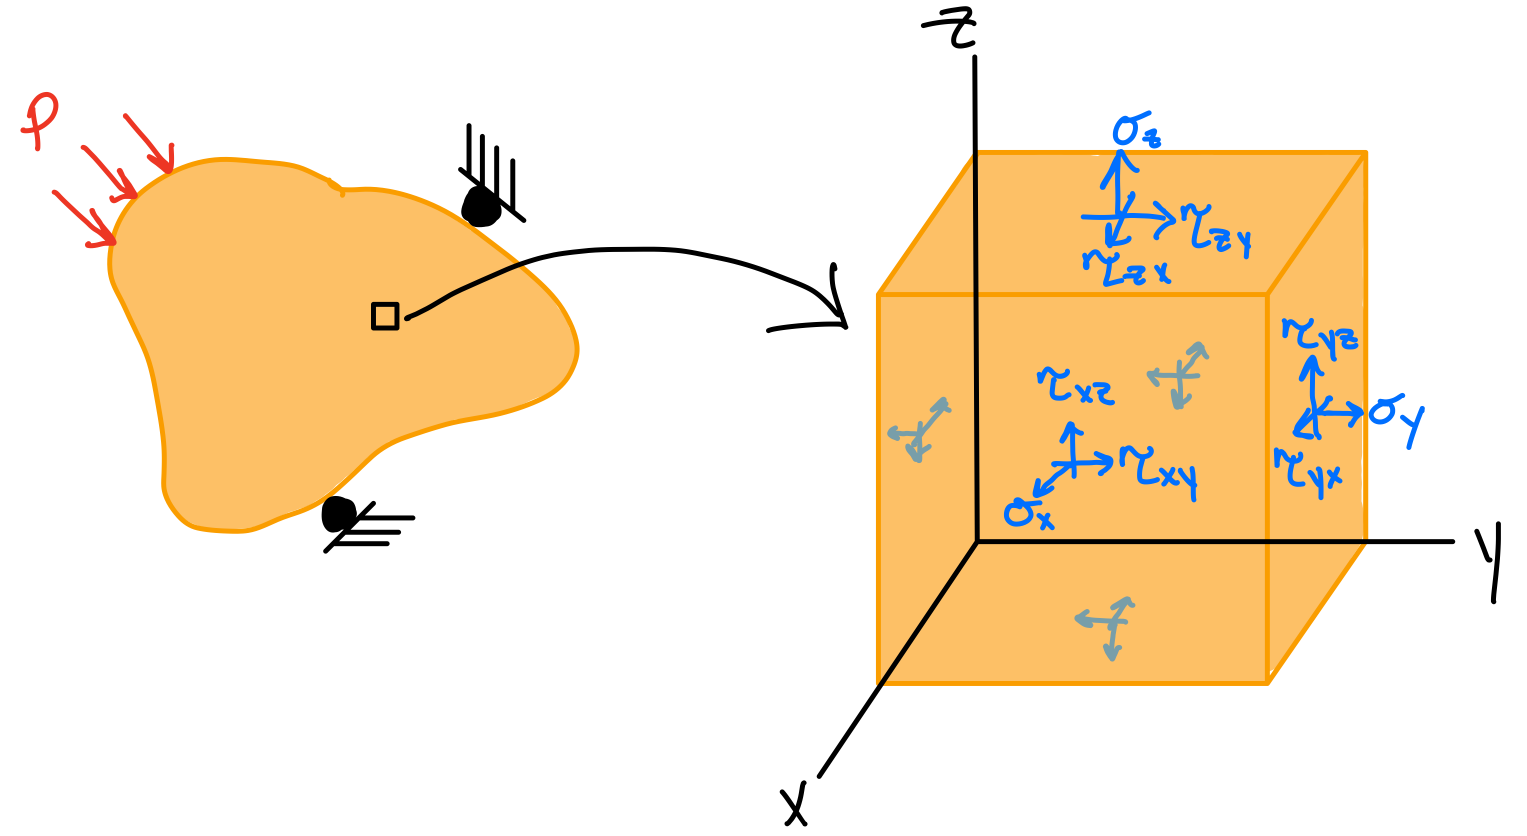
\includegraphics[angle=0, width=5in]{Stress Transformation-Figures/General Stress State.png}
\vspace{-2mm}
\caption{\small \blue{Taken from TAM251 Lecture Notes - L9S2}}
\vspace{-3mm}
\label{Fig:GenStress}
\end{figure*}

\[\boldsymbol{T}=
\begin{bmatrix}
\sigma_{x} & \tau_{xy} & \tau_{xz}\\
\tau_{xy} & \sigma_{y} & \tau_{yz}\\
\tau_{xz} & \tau_{yz} & \sigma_{z}
\end{bmatrix}\]

\noindent \textit{Note:} stress is a physical quantity and as such, it is independent of the chosen coordinate system.

\subsubsection{\blue{Sign Convention}}

\begin{figure*}[!h]
\centering
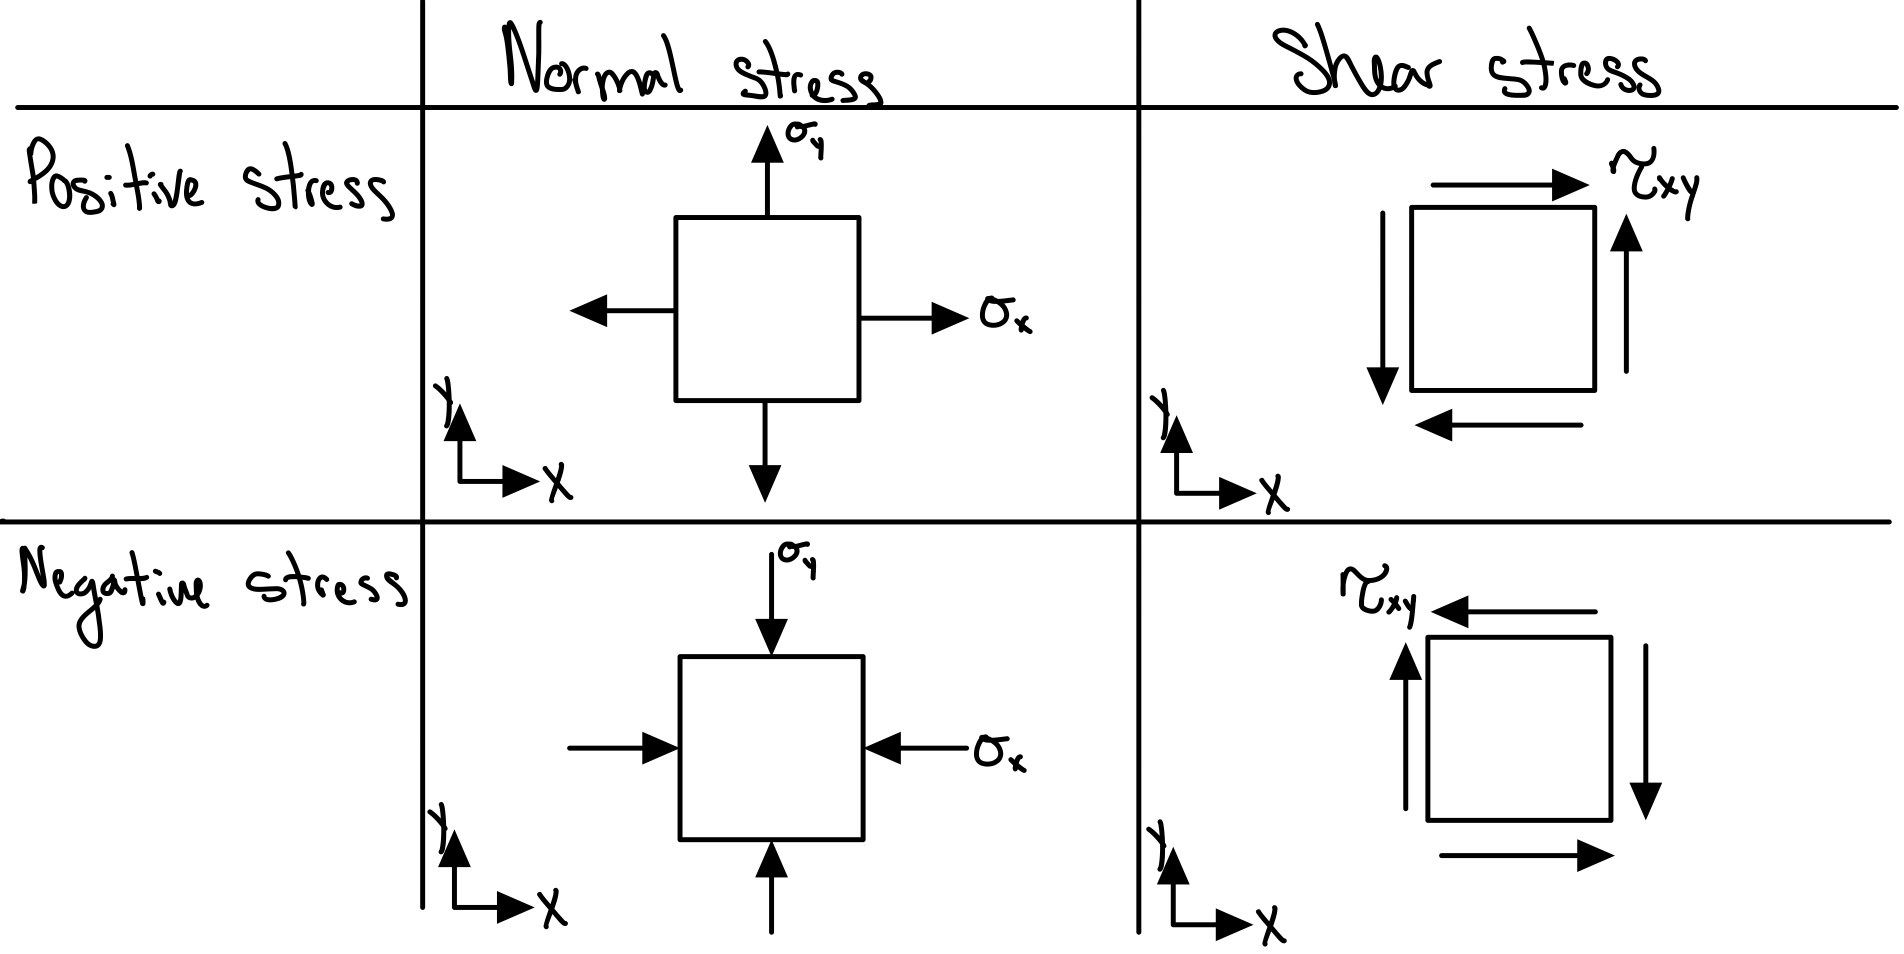
\includegraphics[angle=0, width=3.8in]{Stress Transformation-Figures/Sign Convention.png}
\vspace{-2mm}
\caption{\small \blue{Sign conventions on 2D elements}}
\vspace{-3mm}
\label{Fig:SignConvention}
\end{figure*}

\begin{itemize}
    \item \textbf{Positive} normal stress acts \textbf{outward} from all faces
    \item \textbf{Positive} shear stress points towards the \textbf{positive} axis direction in a \textbf{positive} face
    \item \textbf{Positive} shear stress points towards the \textbf{negative} axis direction in a \textbf{negative} face
    
\end{itemize}

\subsection{\blue{Plane Stress}}

\begin{figure*}[!h]
\centering
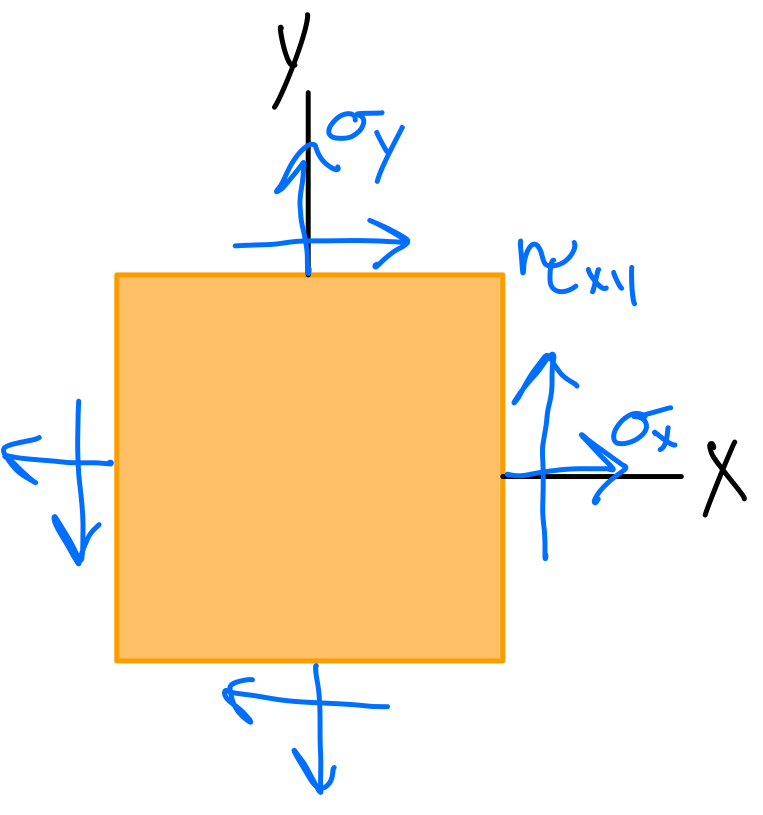
\includegraphics[angle=0, width=1.5in]{Stress Transformation-Figures/Plane Stress.png}
\vspace{-2mm}
\caption{\small \blue{Taken from TAM251 Lecture Notes - L9S5}}
\vspace{-3mm}
\label{Fig:PlaneStress}
\end{figure*}

\noindent Plane stress occurs when two faces of the cube element are stress free.

\[\sigma_{z}=\tau_{zx}=\tau_{zy}=0\]

\noindent \textbf{Example:} Thin plates subject to forces acting in the mid-plane of the plate.

\begin{figure*}[!h]
\centering
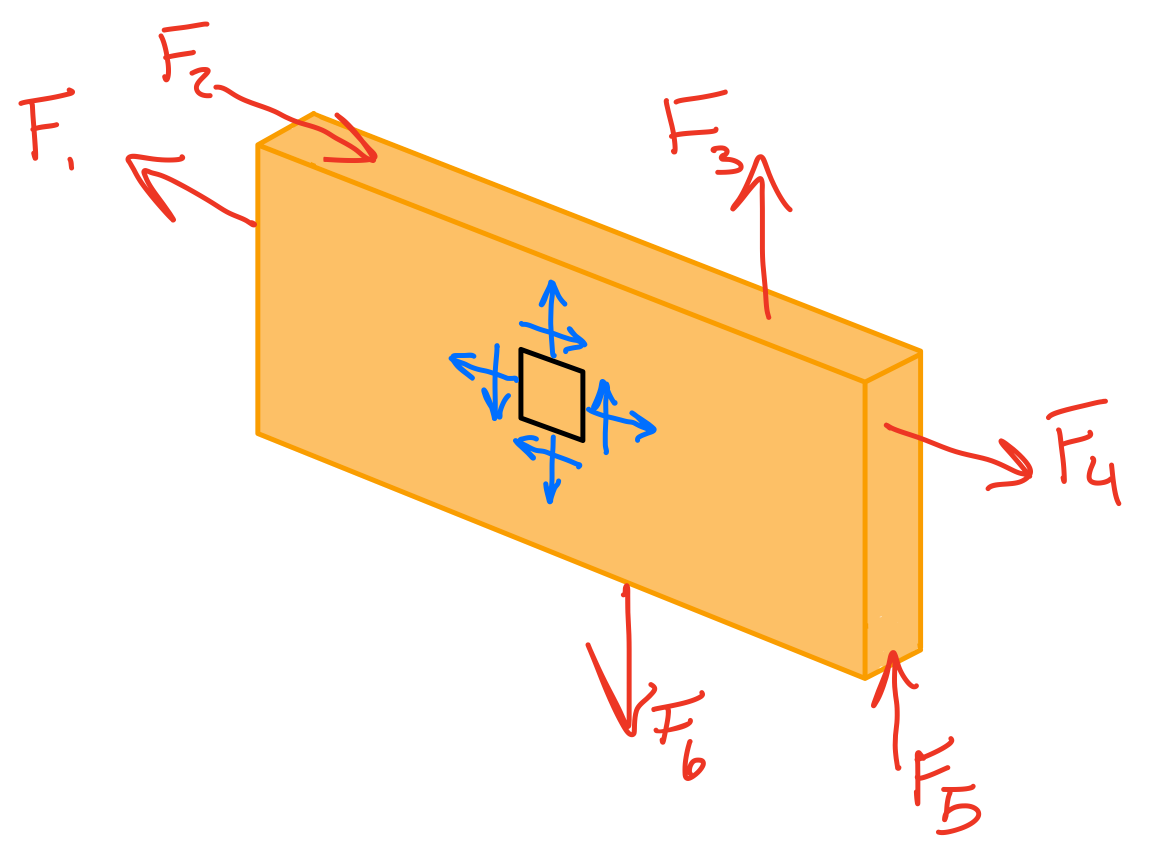
\includegraphics[angle=0, width=2.5in]{Stress Transformation-Figures/Thin Plate.png}
\vspace{-2mm}
\caption{\small \blue{Taken from TAM251 Lecture Notes - L9S3}}
\vspace{-3mm}
\label{Fig:ThinPlate}
\end{figure*}

\subsection{\blue{Plane Stress Transformation}}

For any surface that divides the body ( imaginary or real surface), the action of one part of the body on the other is equivalent to the system of distributed internal forces and moments and it is represented by the stress vector $t^n$ (also called traction), defined on the surface with normal unit vector $n$.

\vspace{5pt}

\noindent The state of stress at a point in the body is defined by all the stress vectors $t^n$ associated with all planes (infinite in number) that pass through that point.

\vspace{5pt}

\noindent Cauchy’s stress theorem states that there exists a stress tensor $T$ (which is independent of $n$), such that $t^n$
 is a linear function of $n$:

\[t^n=\boldsymbol{T}\boldsymbol{n}\]

\noindent We think of stresses acting on faces, so we often associate the state of stress with a coordinate system. However, the selection of a coordinate system is arbitrary (materials don't know about coordinates - it's a mathematical construct!) and we could choose to express the stress state acting on any set of faces aligned with \textbf{any} coordinate system axes. Furthermore, we can relate the states of stress in each coordinate system to one another through \textbf{stress transformation equations.}

\begin{figure*}[!h]
\centering
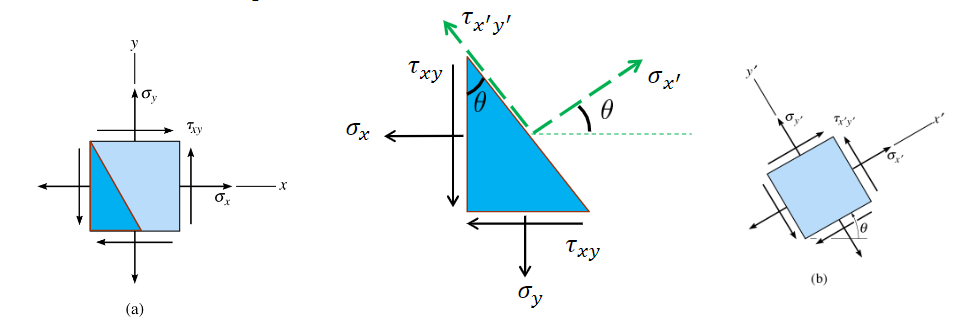
\includegraphics[angle=0, width=5in]{Stress Transformation-Figures/Plane Transformation.png}
\vspace{-2mm}
\caption{\small \blue{Taken from TAM251 Lecture Notes - L9S6}}
\vspace{-3mm}
\label{Fig:PlaneTransform}
\end{figure*}

\subsubsection{Sign Convention}

\begin{itemize}
    \item Both the $x-y$ (original) and $x’-y’$ (transformed) systems follow the right-hand rule.
    \item The orientation of an inclined plane (on which the normal and shear stress components are to be determined) will be defined using the angle $\theta$. The angle $\theta$ is measured from the positive $x$ to the positive $x’$-axis. It is positive if it follows the curl of the right-hand fingers.
\end{itemize}

\[\begin{align}
\sigma_x' &= \frac{\sigma_x + \sigma_y}{2} + \frac{\sigma_x - \sigma_y}{2}\rm\cos(2\theta) + \tau_{xy}\sin(2\theta) \\
\sigma_y' &= \frac{\sigma_x + \sigma_y}{2} - \frac{\sigma_x - \sigma_y}{2}\rm\cos(2\theta) - \tau_{xy}\sin(2\theta) \\
\tau_{x'y'} &= -\frac{\sigma_x - \sigma_y}{2}\rm\sin(2\theta) + \tau_{xy}\cos(2\theta)
\end{align}\]

\noindent \textbf{**Expandable Derivation**}

\vspace{5pt}

\noindent Using the equations from stress in inclined planes:

\[\begin{align}
\sigma_{x}' &= \sigma_{x} \cos ^2(\theta) + 2 \,\tau_{xy} \sin(\theta) \cos(\theta)+\sigma_{y} \sin ^2(\theta) \\
\tau_{x'y'} &= (\sigma_{y} - \sigma_{x}) \sin(\theta) \cos(\theta) + \tau_{xy} ( \cos^2(\theta) - \sin^2(\theta) )
\end{align}\]
                    
\noindent We use the following trigonometric relations:

\[\begin{matrix}
\rm\cos^2\theta = \frac{1 + \rm\cos(2\theta)}{2} & \rm\sin(2\theta) = 2\rm\sin\theta\rm\cos\theta \\
\rm\sin^2\theta = \frac{1 - \rm\cos(2\theta)}{2} & \rm\cos(2\theta) = \rm\cos^2\theta - \rm\sin^2\theta
\end{matrix}\]

\noindent Plugging these in we get:

\[\begin{align}
\sigma_{x}' &= \sigma_{x} \frac{1 + \rm\cos(2\theta)}{2} + \tau_{xy} \sin(2\theta) + \sigma_{y} \frac{1 - \rm\cos(2\theta)}{2} \\
\tau_{x'y'} &= (\sigma_{y} - \sigma_{x}) \frac{\sin(2\theta)}{2} + \tau_{xy} (\frac{1 + \rm\cos(2\theta)}{2} - \frac{1 - \rm\cos(2\theta)}{2})
\end{align}\]

\noindent Rearranging terms:

\[\begin{align}
\sigma_{x}' &= \frac{\sigma_{x}}{2} + \frac{\sigma_{x}\rm\cos(2\theta)}{2} + \frac{\sigma_{y}}{2} - \frac{\sigma_{y}\rm\cos(2\theta)}{2} + \tau_{xy}\sin(2\theta) \\
\tau_{x'y'} &= -\frac{(\sigma_{x} - \sigma_{y})}{2}\sin(2\theta) + (\frac{\tau_{xy}}{2} + \frac{\tau_{xy}\rm\cos(2\theta)}{2} - \frac{\tau_{xy}}{2} + \frac{\tau_{xy}\rm\cos(2\theta)}{2})
\end{align}\]

\noindent We can then simplify to the equations above. Note that to derive $\sigma '_y$, we use the fact that:

\[\sigma_{x}' + \sigma_{y}' = \sigma_{x} + \sigma_{y}\]

\noindent \textbf{**End Derivation**}

\subsubsection{\blue{Stresses in Inclined Planes - moved from stresses page}}

\noindent The relations above are observed only on planes perpendicular to the axis of the member or connection

\begin{align}
\sigma_n &= {\bf n}\cdot\ {\bf t}^{n}={\bf n}\cdot\ {\bf T}\,{\bf n} = \sigma_{x} \cos ^2(\theta) + 2 \,\tau_{xy} \sin(\theta) \cos(\theta)+\sigma_{y} \sin ^2(\theta) \\
\tau_{ns} &= {\bf s}\cdot\ {\bf t}^{n}={\bf s}\cdot\ {\bf T}\,{\bf n} = (\sigma_y - \sigma_{x}) \sin(\theta) \cos(\theta) + \tau_{xy} ( \cos^2(\theta) - \sin^2(\theta) )
\end{align}\

%\[\begin{align}
%\sigma_n &= {\bf n}\cdot\ {\bf t}^{n}={\bf n}\cdot\ {\bf T}\,{\bf n} = \sigma_{x} \cos ^2(\theta) + 2 \,\tau_{xy} \sin(\theta) \cos(\theta)+\sigma_{y} \sin ^2(\theta) \\
%\tau_{ns} &= {\bf s}\cdot\ {\bf t}^{n}={\bf s}\cdot\ {\bf T}\,{\bf n} = (\sigma_y - \sigma_{x}) \sin(\theta) \cos(\theta) + \tau_{xy} ( \cos^2(\theta) - \sin^2(\theta) )
%\end{align}\]

\noindent \textbf{*Expandable derivation*}

\[\sum F_x: -\sigma_x (A\rm\cos\theta) - \tau_{xy}(A\rm\sin\theta) + (\sigma_{x}'\rm\cos\theta)A - (\tau_{x'y'}\rm\sin\theta)A=0\]
\[\sum F_y: -\sigma_y (A\rm\sin\theta) - \tau_{xy}(A\rm\cos\theta) + (\sigma_{x}'\rm\sin\theta)A - (\tau_{x'y'}\rm\cos\theta)A=0\]

\noindent Rearrange terms:

\[A[\sigma_{x}'\rm\cos\theta - \tau_{x'y'}\rm\sin\theta] = A[\sigma_{x}\rm\cos\theta + \tau_{xy}\rm\sin\theta]\]
\[A[\sigma_{x}'\rm\sin\theta - \tau_{x'y'}\rm\cos\theta] = A[\sigma_{x}\rm\sin\theta + \tau_{xy}\rm\cos\theta]\]

\noindent Combine into a matrix:

\[\begin{bmatrix}
\rm\cos\theta & -\rm\sin\theta \\
\rm\sin\theta & \rm\cos\theta
\end{bmatrix}
\begin{bmatrix}
\sigma_{x}' \\
\tau_{x'y'}
\end{bmatrix} =
\begin{bmatrix}
\sigma_{x}\rm\cos\theta & \tau_{xy}\rm\sin\theta \\
\sigma_{y}\rm\sin\theta & \tau_{xy}\rm\cos\theta
\end{bmatrix}
\]
        
\noindent Multiply by the inverse:

\[\begin{bmatrix}
\sigma_{x}' \\
\tau_{x'y'}
\end{bmatrix} =
\begin{bmatrix}
\rm\cos\theta & \rm\sin\theta \\
-\rm\sin\theta & \rm\cos\theta
\end{bmatrix}
\begin{bmatrix}
\sigma_{x}\rm\cos\theta & \tau_{xy}\rm\sin\theta \\
\sigma_{y}\rm\sin\theta & \tau_{xy}\rm\cos\theta
\end{bmatrix}
\]

\noindent \textbf{**End Derivation**}

\subsubsection{\blue{Torsion in Inclined Planes - moved from torsion page - should this go under the max shear stress subsection?}}

\noindent Recall projected forces:

\[\sigma_n = \frac{P}{A_o}(\cos^2(\theta))\] 
\[\tau_{ns} = -\frac{P}{A_o}\sin(\theta)\cos(\theta)\]

\noindent Maximum normal stress at 90 degrees: 
\begin{figure*}[!h]
\centering
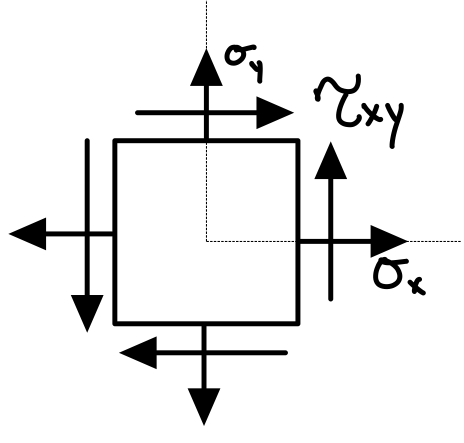
\includegraphics[angle=0, width=2.25in]{Stress Transformation-Figures/Max Normal.png}
\vspace{-2mm}
\caption{\small \blue{Max normal stress}}
\vspace{-3mm}
\label{Fig:MaxNormal}
\end{figure*}


\noindent Maximum shear stress at 45 degrees: \begin{figure*}[!h]
\centering
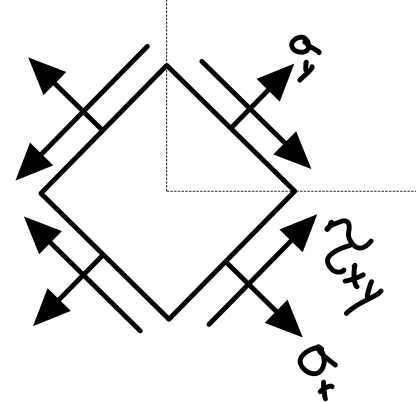
\includegraphics[angle=0, width=2in]{Stress Transformation-Figures/Max Shear.png}
\vspace{-2mm}
\caption{\small \blue{Max shear stress}}
\vspace{-3mm}
\label{Fig:MaxShear}
\end{figure*}

\noindent A circular shaft under torsion develops PURE SHEAR on cross sections between longitudinal planes (the faces of element $a$ are parallel and perpendicular to the axis of the shaft) \begin{figure*}[!h]
\centering
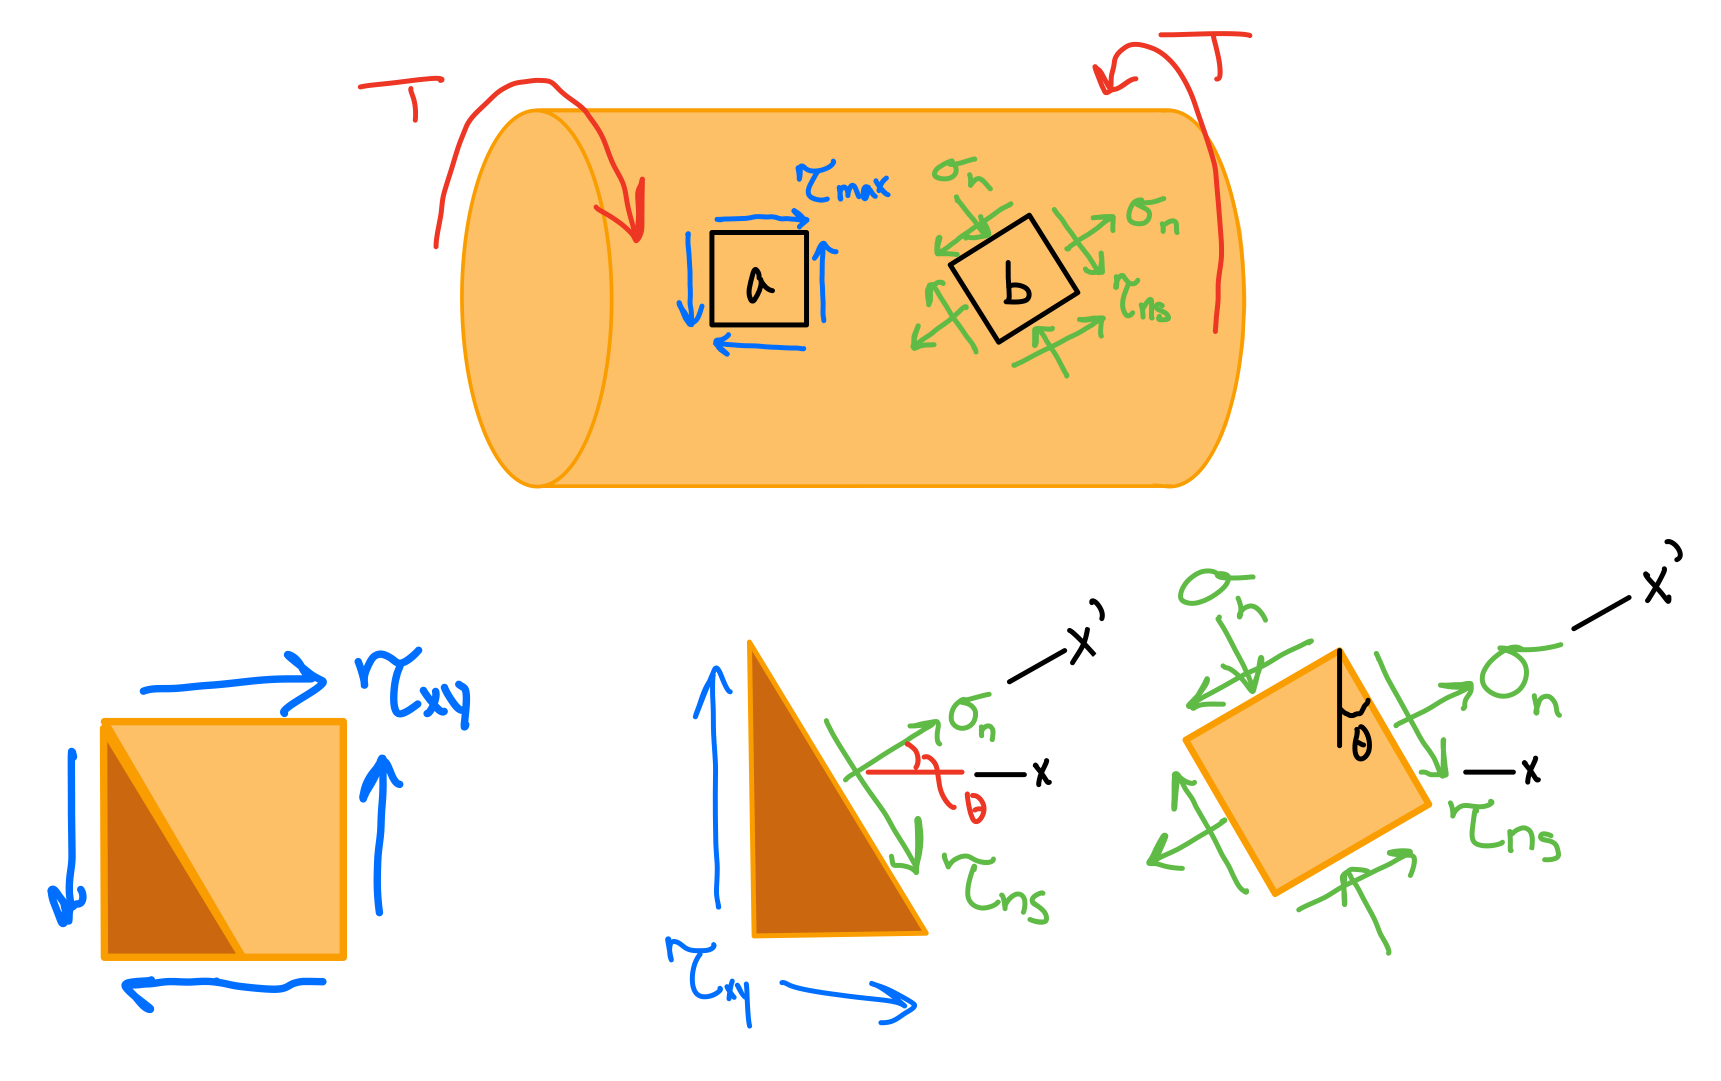
\includegraphics[angle=0, width=3in]{Stress Transformation-Figures/Circular Shaft Torsion.png}
\vspace{-2mm}
\caption{\small \blue{Taken from TAM251 Lecture Notes - L9S19}}
\vspace{-3mm}
\label{Fig:MaxNormal}
\end{figure*}

\[\sigma_n = 2\tau_{max} \sin\theta \cos\theta = \tau_{max} \sin (2\theta)\] 
\[\tau_{ns} = \tau_{max}(\cos^2\theta - \sin^2\theta) = \tau_{max} \cos(2\theta)\]

\begin{figure*}[!h]
\centering
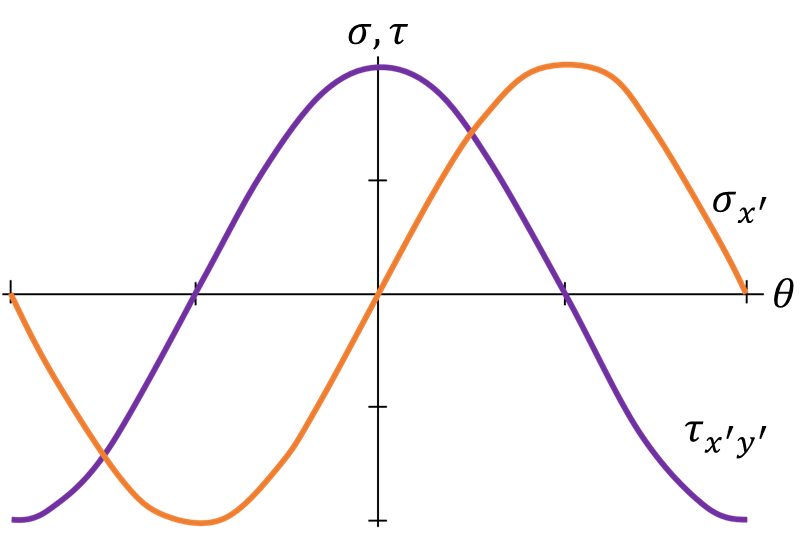
\includegraphics[angle=0, width=3in]{Stress Transformation-Figures/normalShearStressRelation.png}
\vspace{-2mm}
\caption{\small From ref pages}
\vspace{-3mm}
\label{Fig:StressRelation}
\end{figure*}

\noindent Maximum normal stress at:

\[\sigma_n = \tau_{max} = \frac{Tc}{J}\] 
\[\sigma_s = -\tau_{max} = -\frac{Tc}{J}\] 
\[\tau_{ns} = 0\]

\noindent Maximum shear stress at:

\[\sigma_n = 0\] 
\[\sigma_s = 0\] 
\[\tau_{ns} = \tau_{max} = \frac{Tc}{J}\]


\subsection{\blue{Principal Stresses}}

\begin{figure*}[!h]
\centering
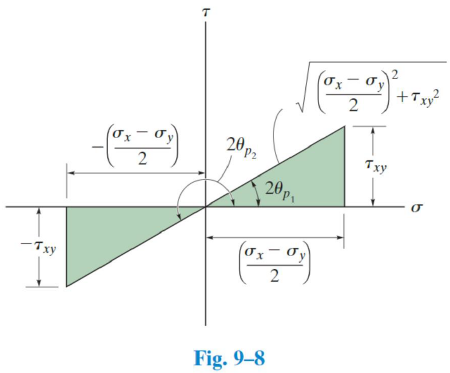
\includegraphics[angle=0, width=3.5in]{Stress Transformation-Figures/Principle Stresses.png}
\vspace{-2mm}
\caption{\small \blue{Taken from TAM251 Lecture Notes - L9S10}}
\vspace{-3mm}
\label{Fig:PrinStress}
\end{figure*}

\noindent The angle at which $\sigma_{x}'$ is maximized is:

\[\rm\tan(2\theta_{p1}) = \frac{2\tau_{xy}}{\sigma_x - \sigma_y}\]
\[\theta_{p2} = \theta_{p1} + 90^o\]

\noindent \textbf{**Expandable Derivation**}

\noindent Recall that: 

\[\sigma_x' = \frac{\sigma_x + \sigma_y}{2} + \frac{\sigma_x - \sigma_y}{2}\rm\cos(2\theta) + \tau_{xy}\sin(2\theta)\]

\noindent To maximize an equation, we take the derivative and set it equal to zero:

\[\frac{d\sigma_{x}'}{d\theta} = -2\rm\sin(2\theta)[\frac{\sigma_x-\sigma_y}{2}] + 2\rm\cos(2\theta)\tau_{xy} = 0 \]

\[(\sigma_x - \sigma_y)\rm\sin(2\theta) = 2\tau_{xy}\rm\cos(2\theta)\]

\[\tan(2\theta) = \frac{2\tau_{xy}}{\sigma_x - \sigma_y}\]
 \noindent \textbf{**End Derivation**}
 
\noindent The maximum/minimum normal stress values (the principal stresses) associated with $\theta_{p1}$ and $\theta_{p2}$ are:

\[\sigma_{1,2} = \frac{\sigma_x +\sigma_y}{2} \pm \sqrt{(\frac{\sigma_x - \sigma_y}{2})^2 + \tau_{xy}^2}\]

\noindent We use the convention that $\sigma_1 > \sigma_2$

\begin{figure*}[!h]
\centering
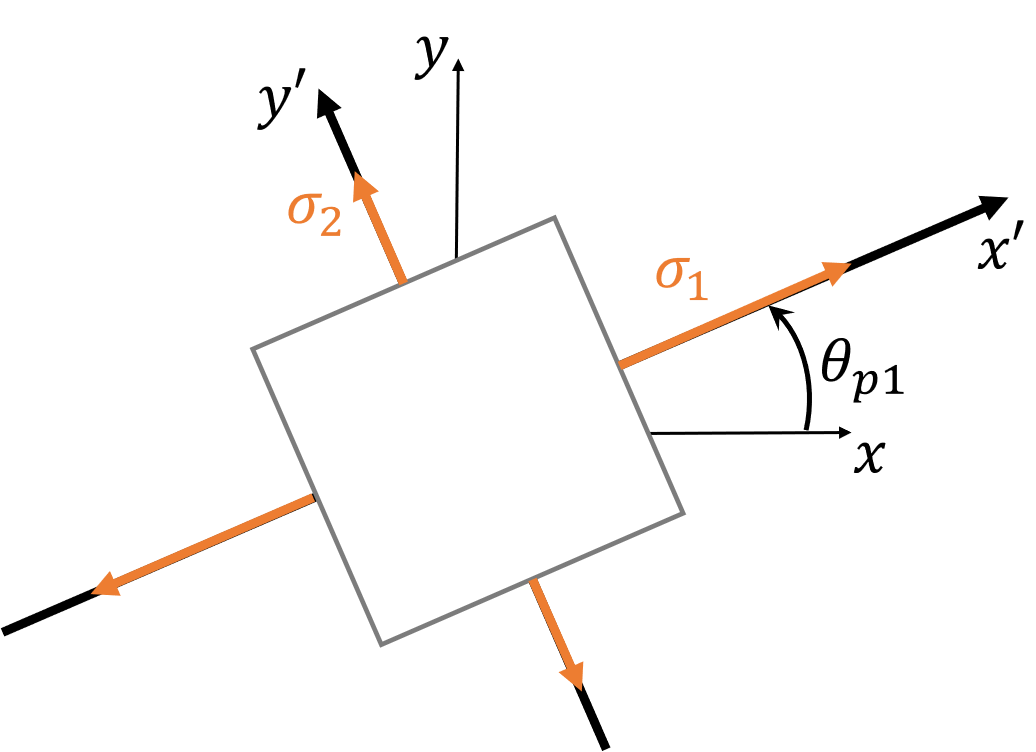
\includegraphics[angle=0, width=3in]{Stress Transformation-Figures/principalStressesElement.png}
\vspace{-2mm}
\caption{\small from ref pages}
\vspace{-3mm}
\label{Fig:PrinStressElem}
\end{figure*}

\subsubsection{Alternative Approach: Eigenvalues}

The stress tensor is a physical quantity and therefore independent of the coordinate system. There are certain invariants associated with every tensor which are also independent of the coordinate system.

\begin{itemize}
    \item First-order tensors (vectors): \textbf{magnitude} is the invariant of a vector, since it is independent of the coordinate system chosen to represent the vector.
    \item Second-order tensors (matrices): three independent invariant quantities associated with it. One set of such invariants are the \textbf{eigenvalues} of the stress tensor, which are called the principal stresses. The \textbf{eigenvectors} define the principal direction vectors.
\end{itemize}

\noindent Because of symmetry, the stress tensor T has real eigenvalues $\lambda$ and mutually perpendicular eigenvectors $v$ such that

\[Tv = \lambda v \rightarrow (T-\lambda I)v = 0\]

\noindent From linear algebra we know that a system of linear equations $A v = 0$ has a non-zero solution $\boldsymbol{v}$ if, and only if, the determinant of the matrix $\boldsymbol{A}$ is zero, that is:

\[\det(\boldsymbol{T}-\lambda\boldsymbol{I})=0\]

\noindent \textbf{**Expandable Derivation**}

\noindent Expanding this equation we get:

\[\det\Biggl(\begin{bmatrix}
\sigma_{x} & \tau_{xy}\\
\tau_{xy} & \sigma_{y}
\end{bmatrix}
- \begin{bmatrix}
\lambda & 0\\
0 & \lambda
\end{bmatrix}
\Biggr) = 0
\]
\[\det\Biggl(\begin{bmatrix}
\sigma_{x}-\lambda & \tau_{xy}\\
\tau_{xy} & \sigma_{y}-\lambda
\end{bmatrix}
\Biggr) = 0
\]
                      
\noindent We evaluate the determinate:

\[(\sigma_{x}-\lambda)(\sigma_{y}-\lambda) - \tau_{xy}^2 = 0\]
\[\sigma_{x}\sigma_{y} - \lambda\sigma_{y} -\lambda\sigma_{x} + \lambda^2 - \tau_{xy}^2 = 0\]
                      
\noindent Rearranging we get:

\[\lambda^2 - \lambda(\sigma_{y} + \sigma_{x}) + \sigma_{x}\sigma_{y} - \tau_{xy}^2 = 0\]

\noindent Now we can solve for the eigenvalues using the quadratic equation where $\rm\ a = 1$, $\rm\ b = -(\sigma_{y} + \sigma_{x})$, and $\rm\ c = \sigma_{x}\sigma_{y} - \tau_{xy}^2$


\[\begin{align}
\lambda &= \frac{(\sigma_{y} + \sigma_{x}) \pm \sqrt{(\sigma_{y} + \sigma_{x})^2 - 4(\sigma_{x}\sigma_{y} - \tau_{xy}^2)}}{2} \\
&= \frac{(\sigma_{x} + \sigma_{y})}{2} \pm \frac{\sqrt{\sigma_{y}^2 + 2\sigma_{y}\sigma_{x} + \sigma_{x}^2 - 4\sigma_{x}\sigma_{y} + 4\tau_{xy}^2}}{2} \\
&= \frac{(\sigma_{x} + \sigma_{y})}{2} \pm \frac{\sqrt{\sigma_{y}^2 - 2\sigma_{y}\sigma_{x} + \sigma_{x}^2 + 4\tau_{xy}^2}}{2} \\
&= \frac{(\sigma_{x} + \sigma_{y})}{2} \pm \sqrt{\frac{(\sigma_{y} - \sigma_{x})^2 + 4\tau_{xy}^2}{4}} \\
&= \frac{(\sigma_{x} + \sigma_{y})}{2} \pm \sqrt{\biggl(\frac{\sigma_{y} - \sigma_{x}}{2}\biggr)^2 + \tau_{xy}^2}
\end{align}\]

 \noindent This is the same result as the geometric derivation above, thus $\lambda_{1,2} = \sigma_{1,2}$.                     

\vspace{5pt}

\noindent \textbf{**End Derivation**}

\vspace{5pt}

\noindent \textbf{**Expandable Derivation**}

\vspace{5pt}

\noindent To find the eigenvectors, we plug our eigenvalues back into the equation $(\boldsymbol{T}-\lambda\boldsymbol{I})\boldsymbol{v} = 0$. We will start with the first eigenvalue, $\lambda_1 = \sigma_1$:

\[\begin{bmatrix}
\sigma_{x}-\sigma_{1} & \tau_{xy}\\
\tau_{xy} & \sigma_{y}-\sigma_{1}
\end{bmatrix}
\begin{bmatrix}
v_{11} \\
v_{12}
\end{bmatrix}
= 0\]
                      
\noindent Multiplying out gives two equations:

\[(\sigma_{x}-\sigma_{1})v_{11} + \tau_{xy}v_{12} = 0\]
\[\tau_{xy}v_{12} + (\sigma_{x}-\sigma_{1})v_{12} = 0\]

                      
\noindent The angle of the eigenvector will be:

\[\theta_{p1} = \tan^{-1}\Bigl(\frac{v_{12}}{v_{11}}\Bigr)\]

\noindent This angle can be derived from both equations, therefore:

\[\theta_{p1} = \tan^{-1}\Bigl(\frac{\sigma_1 - \sigma_x}{\tau_{xy}}\Bigr) = \tan^{-1}\Bigl(\frac{\tau_{xy}}{\sigma_1 - \sigma_y}\Bigr)\]

\noindent We can repeat this procedure for the second eigenvalue, $\lambda_2 = \sigma_2$:

\[\theta_{p2} = \tan^{-1}\Bigl(\frac{\sigma_2 - \sigma_x}{\tau_{xy}}\Bigr) = \tan^{-1}\Bigl(\frac{\tau_{xy}}{\sigma_2 - \sigma_y}\Bigr)\]

\noindent \textbf{**End Derivation**}
 \clearpage
\subsection{\blue{Maximum Shear Stress}}

\begin{figure*}[!h]
\centering
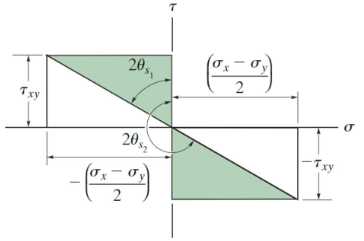
\includegraphics[angle=0, width=3.5in]{Stress Transformation-Figures/Max Shear Stresses.png}
\vspace{-2mm}
\caption{\small \blue{Taken from TAM251 Lecture Notes - L9S13}}
\vspace{-3mm}
\label{Fig:MaxShearStress}
\end{figure*}

\noindent The angle at which $\tau_{x'y'}$ is maximized is:

\[\tan(2\theta_{s1}) = \frac{-(\sigma_x - \sigma_y)}{2\tau_{xy}}\]
\[\theta_{s2} = \theta_{s1} + 90^o\]

\noindent \textbf{**Expandable Derivation**}

\vspace{5pt}

\noindent Recall that:

\[\tau_{x'y'} = -\frac{\sigma_x - \sigma_y}{2}\rm\sin(2\theta) + \tau_{xy}\cos(2\theta)\]

\noindent To maximize an equation, we take the derivative and set it equal to zero:

\[\frac{d\tau_{x'y'}}{d\theta} = -\frac{\sigma_x - \sigma_y}{2}2\rm\cos(2\theta) - \tau_{xy}2\rm\sin(2\theta) = 0\]
\[-2\tau_{xy}\rm\sin(2\theta)  = (\sigma_x - \sigma_y)\rm\cos(2\theta)\]
\[\tan(2\theta) = \frac{-(\sigma_x - \sigma_y)}{2\tau_{xy}}\]

\noindent \textbf{**End Derivation**}

\noindent The maximum/minimum in plane shear stress values associated with $\theta_{s1}$ and $\theta_{s2}$ are:

\[|\tau_{max}| = \sqrt{(\frac{\sigma_x - \sigma_y}{2})^2 + \tau_{xy}^2}\]

\noindent A maximum shear stress element has

\[\sigma_{x}' = \sigma_{y}' = \sigma_{avg} = \frac{\sigma_x + \sigma_y}{2}\]

\noindent \textit{i.e.;} unlike with the principal stress element, the normal stresses are not zero.

\begin{figure*}[!h]
\centering
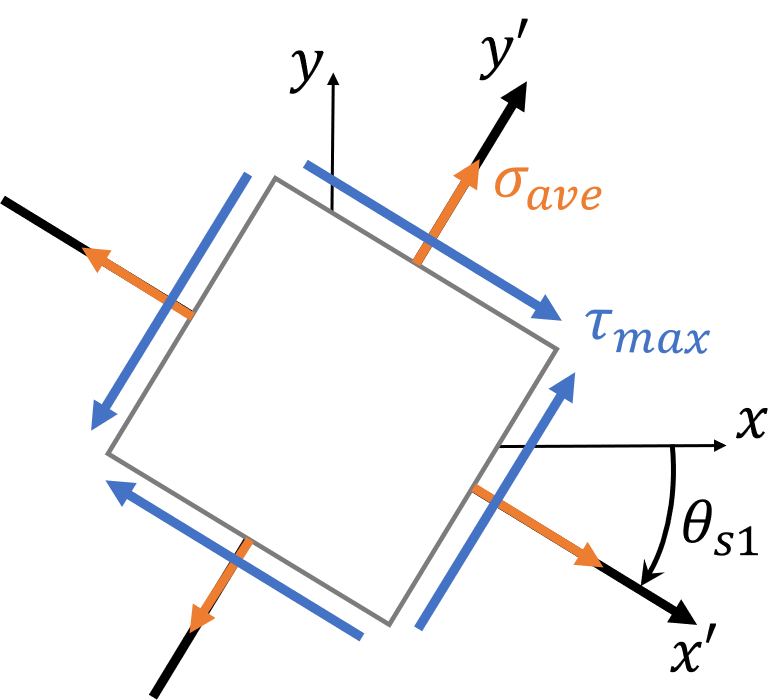
\includegraphics[angle=0, width=2in]{Stress Transformation-Figures/maxShearStressState.png}
\vspace{-2mm}
\caption{\small From ref pages}
\vspace{-3mm}
\label{Fig:MaxShearStressState}
\end{figure*}


\noindent The orientations for the principal stress element and max shear stress element are $45^o$
apart.
 
\subsection{Mohr's Circle}

\begin{figure*}[!h]
\centering
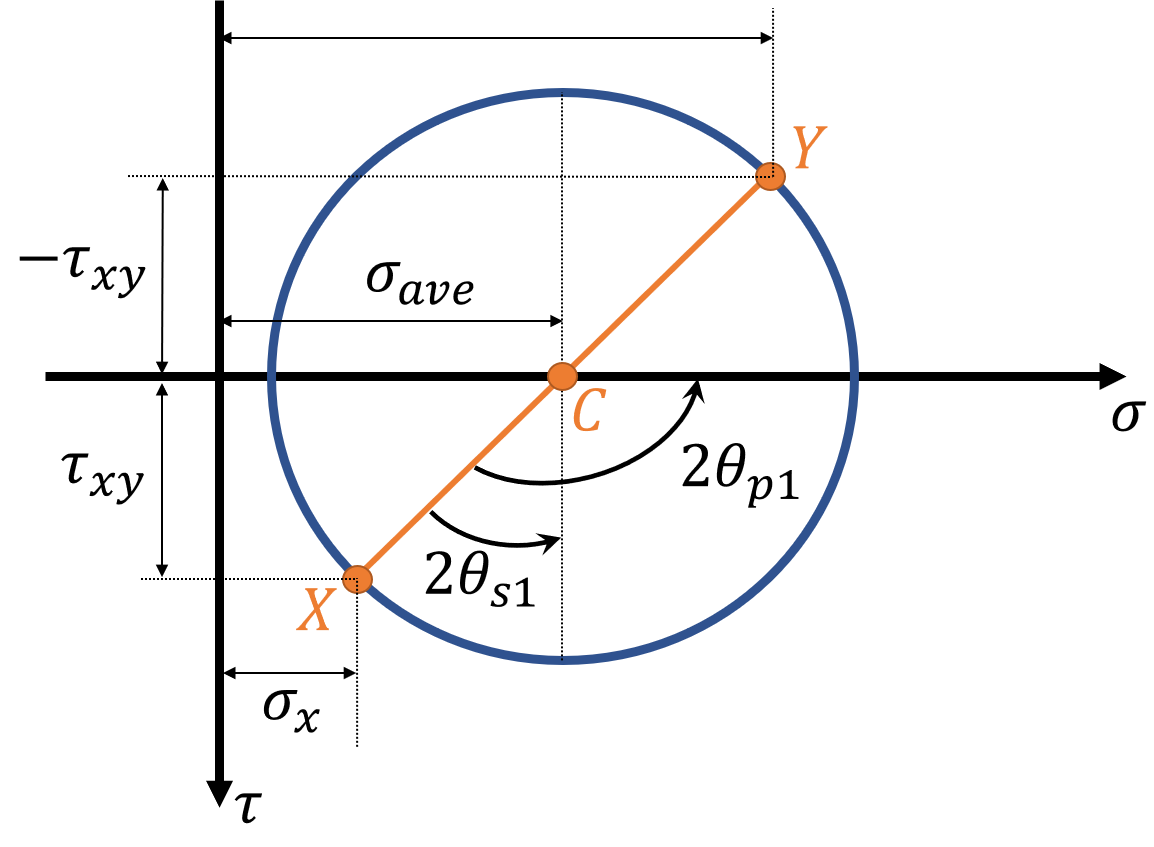
\includegraphics[angle=0, width=2in]{Stress Transformation-Figures/mohrsCircle.png}
\vspace{-2mm}
\caption{\small From ref pages}
\vspace{-3mm}
\label{Fig:MohrCircle}
\end{figure*}

\noindent Mohr's circle is a graphical representation of stress transformations. The equations for stress transformations actually describe a circle if we consider the normal stress $\sigma$ to be the x-coordinate and the shear stress $\pi$ to be the y-coordinate.

\noindent Circle Centroid:

\[C = \sigma_{avg} = \frac{\sigma_x +\sigma_y}{2} = \frac{\sigma_1 +\sigma_2}{2}\]

\noindent Circle Radius:

\[R = \sqrt{(\frac{\sigma_x - \sigma_y}{2})^2 + \tau_{xy}^2}\]

\noindent We classify two points:

\[ \begin{align}
\rm\ Point \ X&: (\sigma_x, \tau_{xy}) \\
\rm\ Point \ Y&: (\sigma_y, -\tau_{xy})
\end{align}\]
                        
\subsection{Interactive: State of Stress}

The state of plane stress at a point on a body is represented by the element below.

\vspace{5pt}

\noindent \textbf{\red{**Interactive element broken**}}

\subsection{Interactive: State of Stress in a Beam}

Let us analyse the stress field in this cantilever beam problem:

\begin{figure*}[!h]
\centering
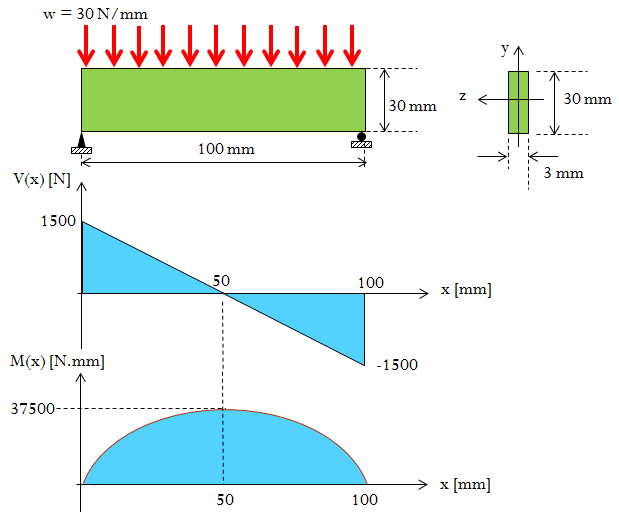
\includegraphics[angle=0, width=3.5in]{Stress Transformation-Figures/CantileverBeam.png}
\vspace{-2mm}
\caption{\small From ref pages}
\vspace{-3mm}
\label{Fig:CantileverBeam}
\end{figure*}

\noindent Choose the coordinates of the point in which you want to obtain the state of plane stress (at the plane z = 0):

\vspace{5pt}

\noindent The state of plane stress at this point is represented by the element below.

\vspace{5pt}

\noindent \textbf{\red{**Interactive element broken**}}